\documentclass[12pt]{article}
\usepackage[utf8]{inputenc}
\newenvironment{sol}[1][Solution]{\begin{trivlist}\item[\hskip\labelsep {\bfseries #1:}]}{\end{trivlist}}
\usepackage[margin=1in]{geometry} 
\usepackage{amsmath,amsthm,amssymb}
\usepackage{color}
\usepackage{minted}
\usepackage{graphicx}
\title{Southern Methodist University \\
Bobby B. Lyle School of Engineering Department of Computer Science \\
Homework 4
}
\usepackage{times,url}   
\author{Operating System and Software System \\
Name: Bingying Liang 
\\ ID: 48999397\\ 
Email: bingyingl@smu.edu \\ 
CS7343 Distance}
\date{Feb 28 2023}

\begin{document}
\maketitle
\begin{itemize}
    \item CS 5343 students must answer exactly 4 questions
    \item CS 7343 students must answer all questions
\end{itemize}
\begin{enumerate}
    \item Consider the following set of processes with the following arrival tome and processing time (i.e. service time).
    \begin{center}
        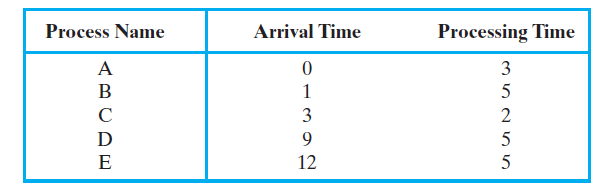
\includegraphics[width=0.6\textwidth]{1.png}
    \end{center}
    Perform the same analysis as depicted in the following table for this set.
    \begin{center}
        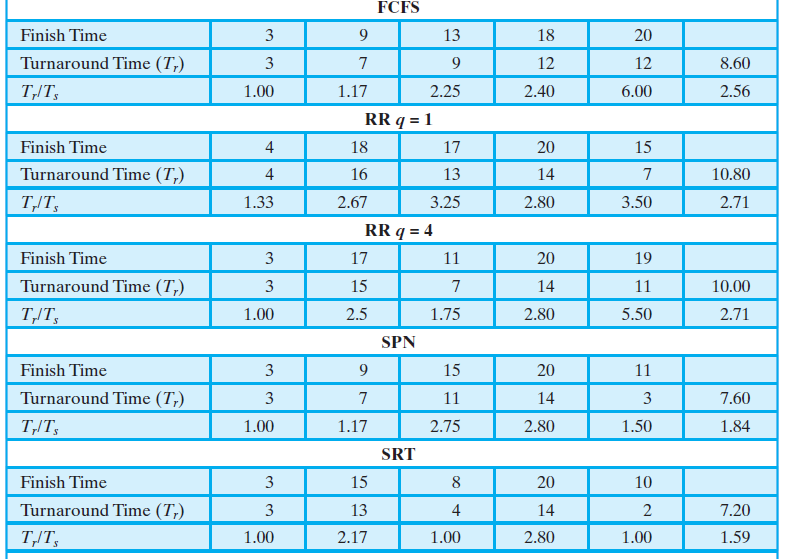
\includegraphics[width=0.8\textwidth]{2.png}
    \end{center}
    \begin{sol}
    \hspace*{\fill}\\
    \begin{center}
        
    \begin{tabular}{|c|c|c|c|c|c|c|}
        \hline
        \multicolumn{7}{|c|}{FCFS}  \\
        \hline 
         Finish Time & 3 & 8 & 10 & 15 & 20 & \\
        \hline
         Turnaround Time ($T_r$) & 3 & 7 & 7 & 6 & 8 & 6.20\\ 
        \hline
         $T_r / T_s$ & 1.00 & 1.40 & 3.50 & 1.20 & 1.60 & 1.74 \\
         \hline
         
        \multicolumn{7}{|c|}{RR $q = 1$}\\
        \hline 
        Finish Time & 6 & 11 & 8 & 18 & 20 & \\
        \hline
         Turnaround Time ($T_r$) & 6 & 10 & 5 & 9 & 8 & 7.60\\ 
        \hline
         $T_r / T_s$ & 2.00 & 2.00 & 2.50 & 1.8 & 1.60 & 1.98 \\
                  \hline


        \multicolumn{7}{|c|}{RR $q = 4$}\\
        \hline 
        Finish Time & 3 & 10 & 9 & 19 & 20 & \\
        \hline
         Turnaround Time ($T_r$) & 3 & 9 & 6 & 10 & 8 & 7.20\\ 
        \hline
         $T_r / T_s$ & 1.00 & 1.80 & 3.00 & 2.00 & 1.60 & 1.88 \\
                  \hline
                  
        \multicolumn{7}{|c|}{SPN}\\
        \hline 
        Finish Time & 3 & 10 & 5 & 15 & 20 & \\
        \hline
         Turnaround Time ($T_r$) & 3 & 9 & 2 & 6 & 8 & 5.60\\ 
        \hline
         $T_r / T_s$ & 1.00 & 1.80 & 1.00 & 1.20 & 1.60 & 1.32 \\
                  \hline
                  
        \multicolumn{7}{|c|}{SRT}\\
        \hline 
        Finish Time & 3 & 10 & 5 & 15 & 20 & \\
        \hline
         Turnaround Time ($T_r$) & 3 & 9 & 2 & 6 & 8 & 5.60\\ 
        \hline
         $T_r / T_s$ & 1.00 & 1.80 & 1.00 & 1.20 & 1.60 & 1.32 \\
                  \hline
        
    \end{tabular}
        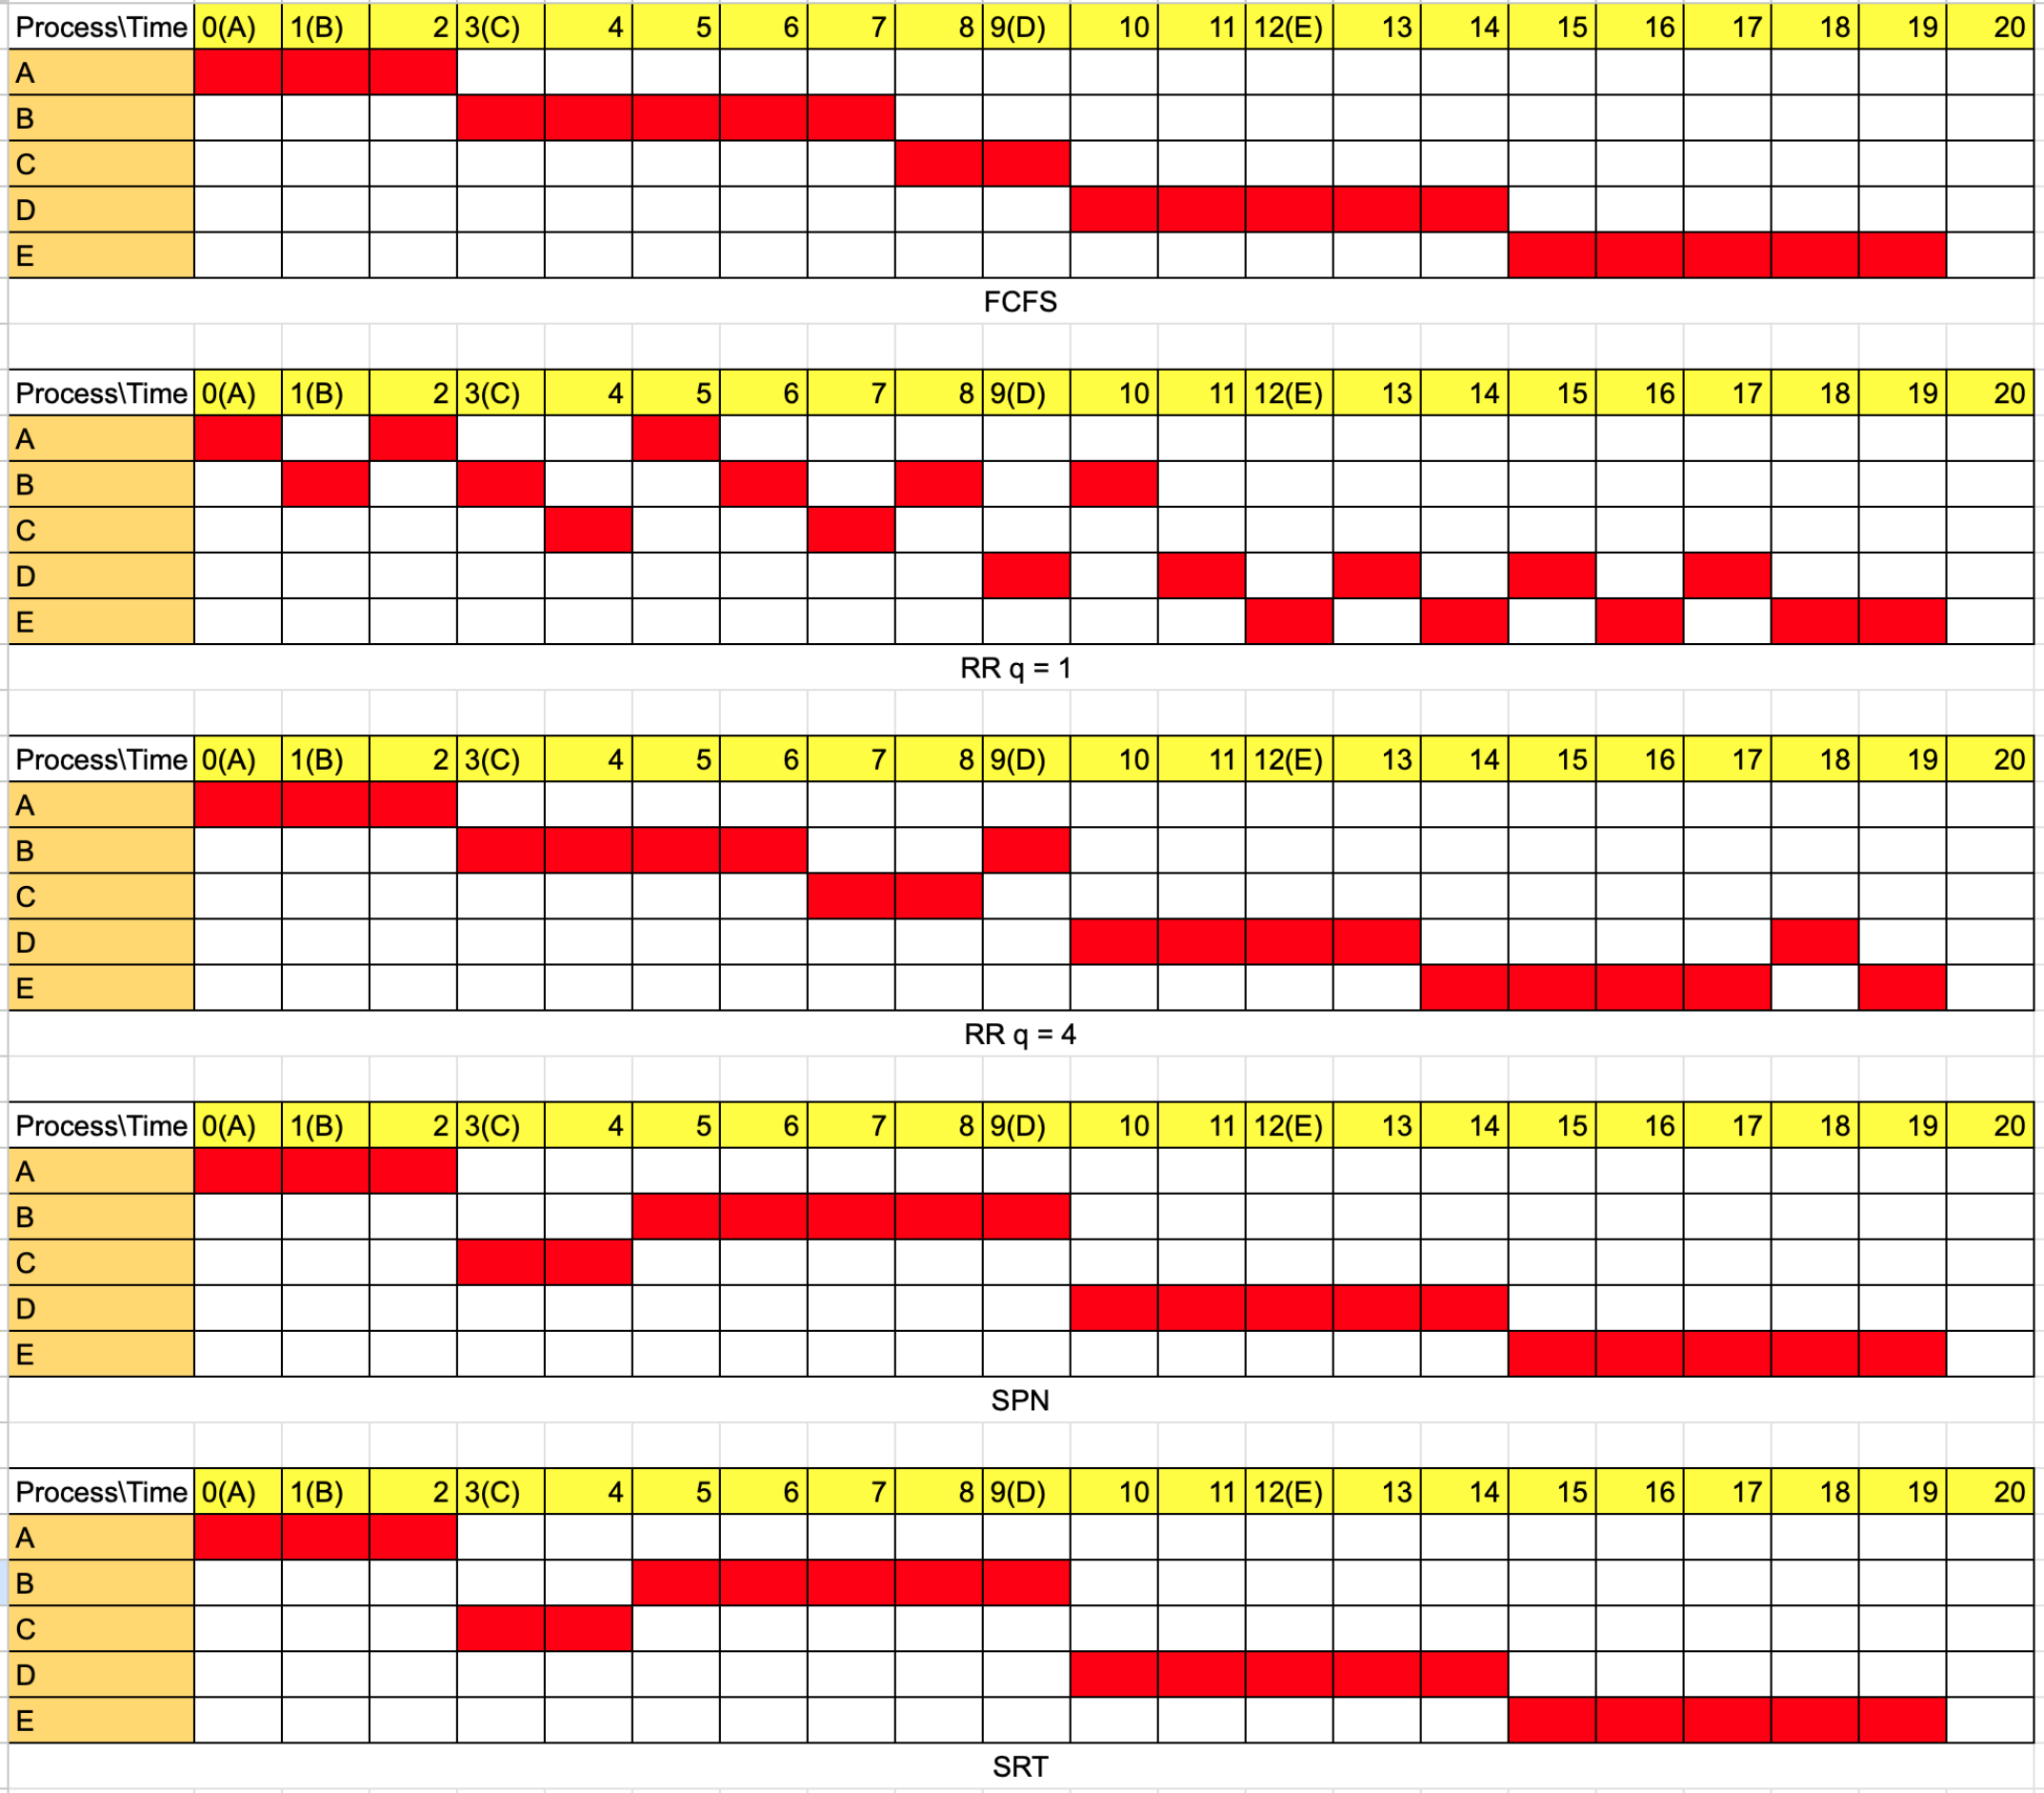
\includegraphics[width=0.9\textwidth]{4.png}

    \end{center}
    \end{sol}
    
    \newpage
    \item Repeat Problem 1 for the following set.
    \begin{center}
        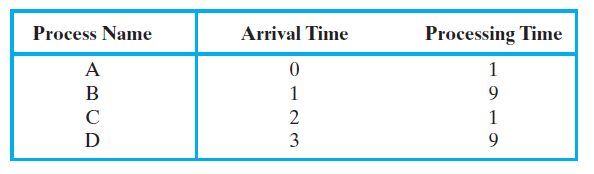
\includegraphics[width=0.6\textwidth]{3.png}
    \end{center}
        \begin{sol}
    \hspace*{\fill}\\
    \begin{center}
        
    \begin{tabular}{|c|c|c|c|c|c|}
        \hline
        \multicolumn{6}{|c|}{FCFS}  \\
        \hline 
         Finish Time & 1 & 10 & 11 & 20 &  \\
        \hline
         Turnaround Time ($T_r$) & 1 & 9 & 9 & 17 & 9.00  \\ 
        \hline
         $T_r / T_s$ & 1.00 & 1.00 & 9.00 & 1.89 & 3.22  \\
         \hline
         
        \multicolumn{6}{|c|}{RR $q = 1$}\\
        \hline 
         Finish Time & 1 & 18 & 3 & 20 &  \\
        \hline
         Turnaround Time ($T_r$) & 1 & 17 & 1 & 17 & 9.00  \\ 
        \hline
         $T_r / T_s$ & 1.00 & 1.89 & 1.00 & 1.89 & 1.44  \\
         \hline
                  
        \multicolumn{6}{|c|}{RR $q = 4$}\\
        \hline 
         Finish Time & 1 & 15 & 6 & 20 &  \\
        \hline
         Turnaround Time ($T_r$) & 1 & 14 & 4 & 17 & 9.00  \\ 
        \hline
         $T_r / T_s$ & 1.00 & 1.56 & 4.00 & 1.89 & 2.11 \\
         \hline
                  
        \multicolumn{6}{|c|}{SPN}\\
        \hline 
         Finish Time & 1 & 10 & 11 & 20 &  \\
        \hline
         Turnaround Time ($T_r$) & 1 & 9 & 9 & 17 & 9.00  \\ 
        \hline
         $T_r / T_s$ & 1.00 & 1.00 & 9.00 & 1.89 & 3.22  \\
         \hline
                  
        \multicolumn{6}{|c|}{SRT}\\
        \hline 
         Finish Time & 1 & 11 & 3 & 20 &  \\
        \hline
         Turnaround Time ($T_r$) & 1 & 10 & 1 & 17 & 7.25  \\ 
        \hline
         $T_r / T_s$ & 1.00 & 1.11 & 1.00 & 1.89 & 1.25  \\
         \hline
        
    \end{tabular}
            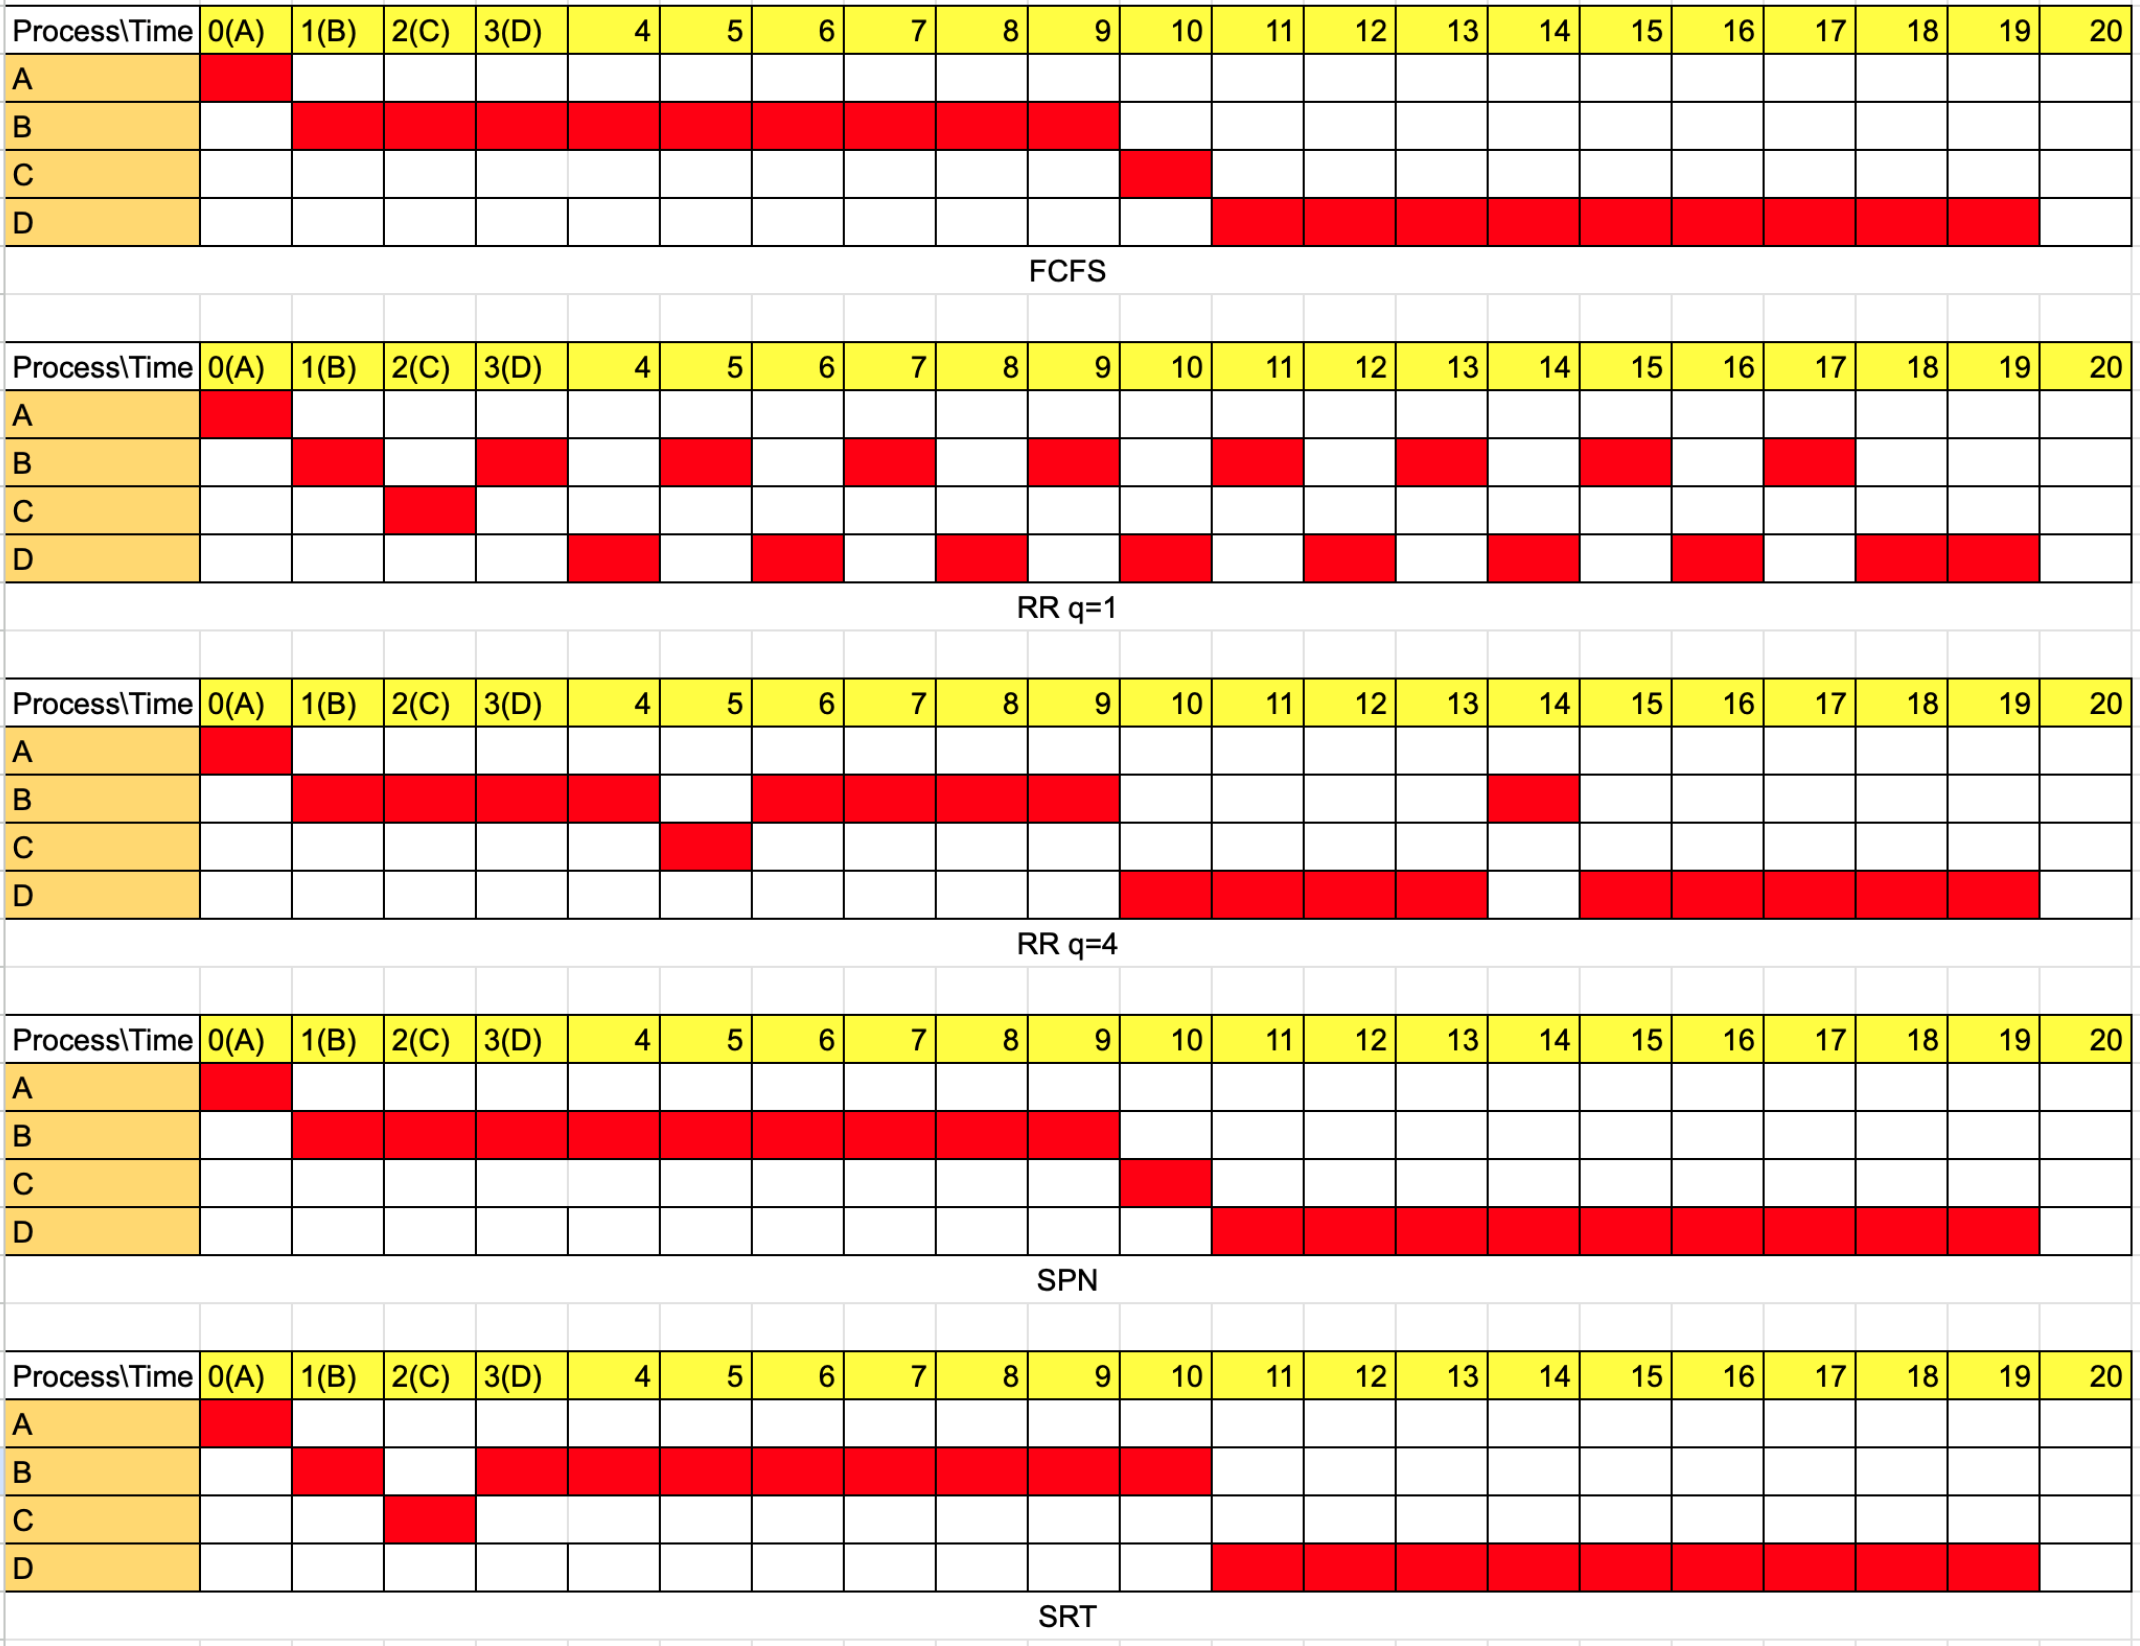
\includegraphics[width=0.9\textwidth]{5.png}
    \end{center}
    \end{sol}
    

    \newpage
    \item Prove (mathematically) or give a correct argument that, among nonpreemptive scheduling algorithms, SPN provides the minimum average waiting time for a batch of jobs that arrive at the same time. Assume that the scheduler must always execute a task if one is available.
    \begin{sol}
        \hspace*{\fill}
        \begin{proof}
            
            \begin{align*}
             & \text{Suppose, there are } n \text{ jobs, and the service time of jobs are } t_1 \leq t_2 \leq \dots \leq t_n.\\
                & \because \text{jobs that arrive at the same time} \\
                & \therefore \text{ For the first job, i.e. job 1, there are } n \text{ jobs are waiting.} \\
                & \therefore \text{ For job 2, there are } n-1 \text{ jobs are waiting.}\\
                & \therefore \text{Average waiting time } = \frac{n t_1+(n-1)t_2+\dots + t_n}{n} \\
                & \text{Suppose, it has other minimum average waiting time, by switching job } i \text{ and } j (i < j).\\
                & \therefore \text{Average waiting time } = \frac{n t_1+(n-1)t_2+\dots + t_n}{n} - \frac{(i-j)(t_i-t_j)}{n}\\
                & \because i < j, t_i<t_j\\
                & \therefore \frac{(i-j)(t_i-t_j)}{n} \leq 0 \\
                & \therefore \frac{n t_1+(n-1)t_2+\dots + t_n}{n} \leq \frac{n t_1+(n-1)t_2+\dots + t_n}{n} - \frac{(i-j)(t_i-t_j)}{n} \\
                & \therefore \text{SPN provides the minimum average waiting time for a batch of jobs that arrive}\\
                & \text{at the same time.}
            \end{align*}
        \end{proof}
    \end{sol}

    \newpage
    \item Most round-robin schedulers use a fixed size quantum. Give an argument in favor of a small quantum. Now give an argument in favor of a large quantum. Compare and contrast the types of systems and jobs to which the arguments apply. Are there any for which both are reasonable?
    \begin{sol}
    \hspace*{\fill}\\
    \textbf{An argument in favor of a small quantum:} Efficiency. The small quantum can increase the responsiveness through frequently running all processes. Especially, the interactive processes in the ready queue. A short quantum is useful for general-purpose computer system. \\
    
    \textbf{An argument in favor of a large quantum:} A large quantum reduces the overhead of process switching, which increase throughput and CPU utilization. It is useful for batch jobs system. \\
    
    \textbf{Both:} There are both are reasonable. We can combine both general-purpose general-purpose system and batch jobs system. For example, some systems might have long jobs but still required just a few user interactions, which means jobs are need a quick response time. Therefore, the quantum of jobs can not be large. In this situation, we can during the time when there is no user interaction, the quantum might be large to increase the throughout, but during the time when there are users interaction, the quantum can be small to increase the responsiveness.





    \end{sol}

    \newpage
    \item An interactive system using round-robin scheduling and swapping tries to give guaranteed response to trivial requests as follows: After completing a round robin cycle among all ready processes, the system determines the time slice to allocate to each ready process for the next cycle by dividing a maximum response time by the number of processes requiring service. Is this a reasonable policy?
    \begin{sol}
    \hspace*{\fill}\\
    This is a reasonable policy as only as there are comparatively few users in the system. Because if there are too much users, with the decreasing time slice, the response times of round-robin scheduling will be increased. Some users might be just need a little service time, but because the long respond times and so many users in the round-robin queue, they have to wait for a quiet long time. And then the processor utilization will decrease. So it is a not reasonable policy when the system has too many users, but it is reasonable when the system just only has comparatively few users.
    
    \end{sol}

    \newpage
    \item Five batch jobs, A through E, arrive at a computer center at essentially the same time. They have an estimated running time of 15, 9, 3, 6, and 12 minutes, respectively. For each of the following scheduling algorithms, determine the turnaround time for each process and the average turnaround for all jobs. Ignore process switching overhead. Explain how you arrived at your answers. 
    \begin{enumerate}
        \item Round robin with a time quantum of 1 minute
        \item FCFS (run in order 15, 9, 3, 6, and 12)
        \item Shortest job first (i.e.  Shortest process next (SPN) 
    \end{enumerate}
    \begin{sol}
    \hspace*{\fill}\\
    (a) Turnaround Time for A, B, C, D, E are 45, 35, 13, 26, and 42 minutes. The average turnaround time is 32.2 minutes.
        \begin{center}
        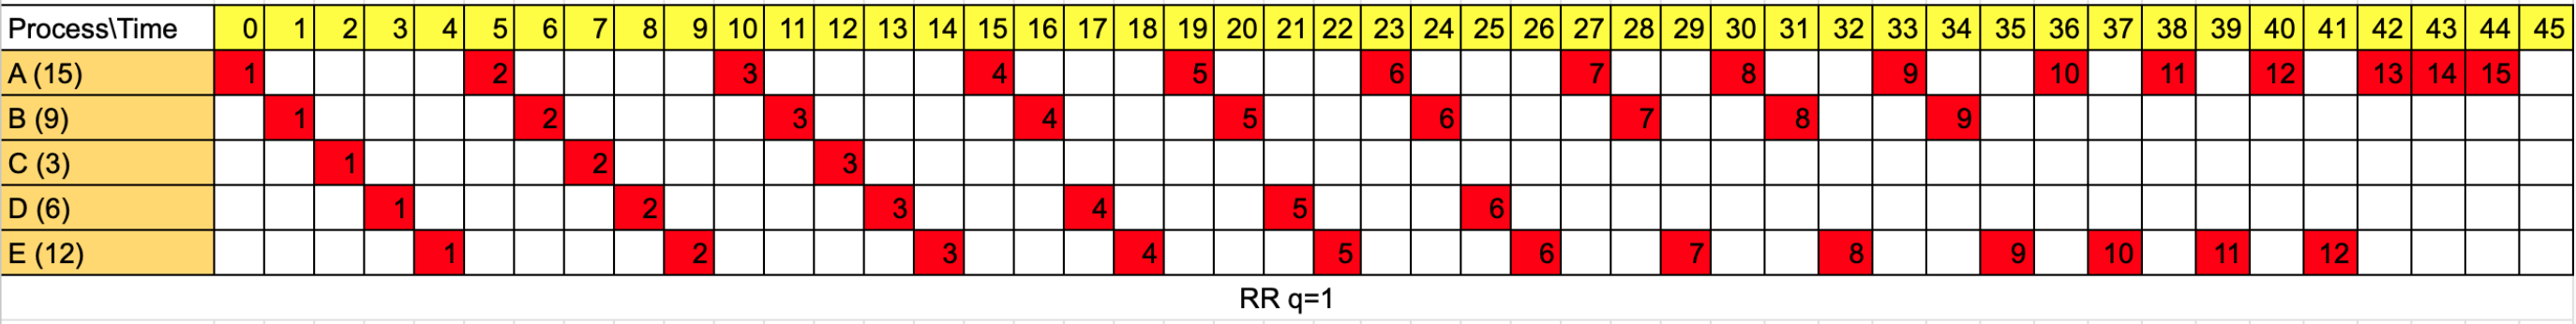
\includegraphics[width=0.9\textwidth]{6.png}
        \begin{tabular}{|c|c|c|c|c|c|c|}
        \hline
        \multicolumn{7}{|c|}{RR $q=1$}  \\
        \hline 
         Arrival time ($T_a$) & 0 & 0 & 0 & 0 & 0 & \\
        \hline
         Finish Time ($T_f$)& 45 & 35 & 13 & 26 & 42 & \\
        \hline
         Turnaround Time ($T_r = T_f - T_a$ )& 45 & 35 & 13 & 26 & 42 & 32.2  \\ 
         \hline
         \end{tabular}
        \end{center}

    (b) Turnaround Time for A, B, C, D, E are 15, 24, 27, 33, and 45 minutes. The average turnaround time is 28.8 minutes.

        \begin{center}
        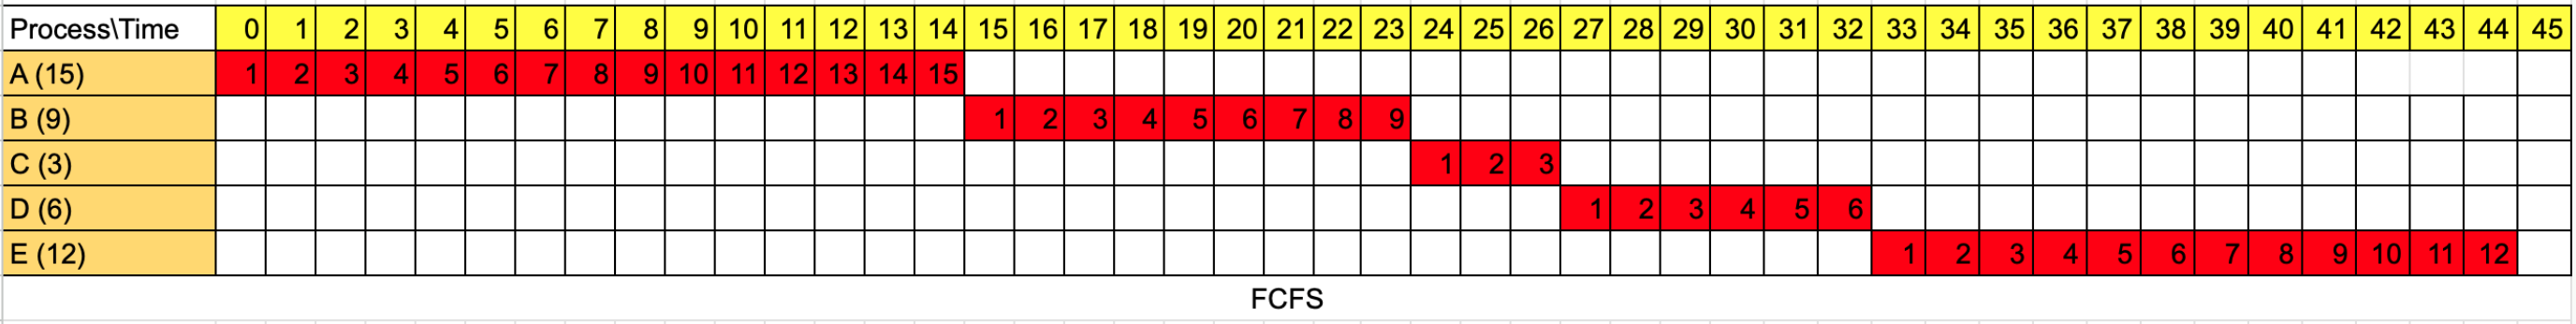
\includegraphics[width=0.9\textwidth]{7.png}
        \begin{tabular}{|c|c|c|c|c|c|c|}
        \hline
        \multicolumn{7}{|c|}{FCFS}  \\
        \hline 
         Arrival time ($T_a$) & 0 & 0 & 0 & 0 & 0 & \\
        \hline
         Finish Time ($T_f$)& 15 & 24 & 27 & 33 & 45 & \\
        \hline
         Turnaround Time ($T_r = T_f - T_a$ ) & 15 & 24 & 27 & 33 & 45 & 28.8  \\ 
         \hline
         \end{tabular}
        \end{center}
        
    (c)  Turnaround Time for A, B, C, D, E are 45, 18, 3, 9, and 30 minutes. The average turnaround time is 21 minutes.

        \begin{center}
        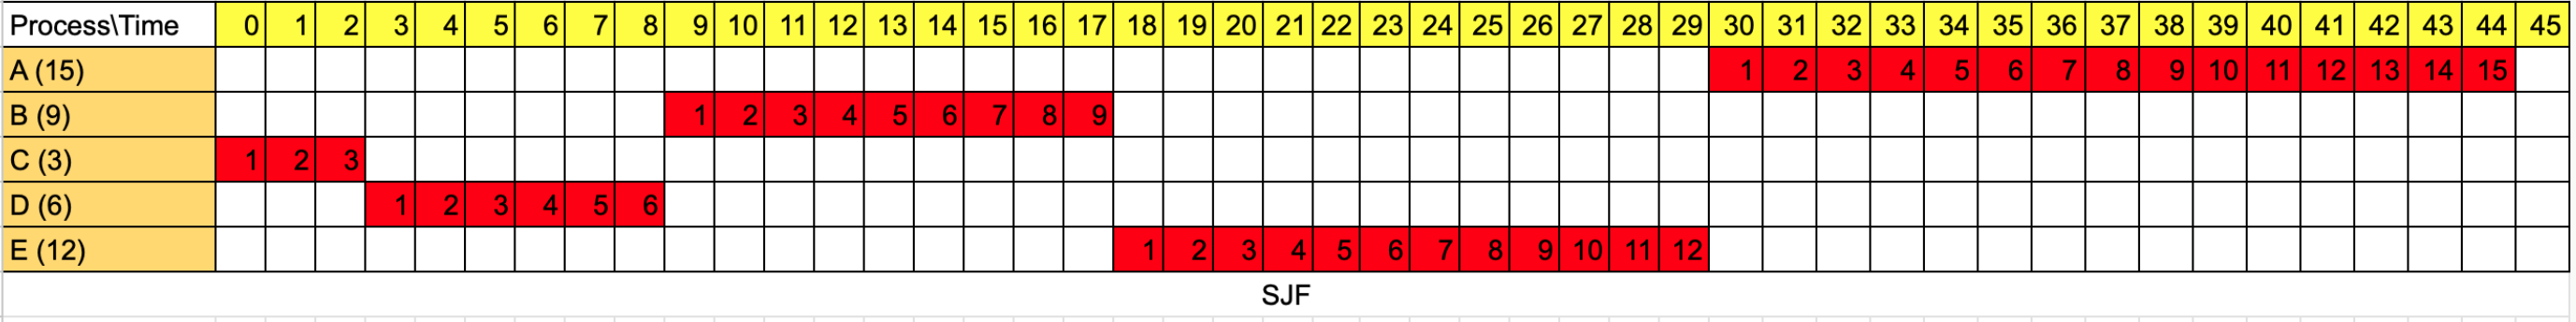
\includegraphics[width=0.9\textwidth]{8.png}
        \begin{tabular}{|c|c|c|c|c|c|c|}
        \hline
        \multicolumn{7}{|c|}{SJF}  \\
        \hline 
         Arrival time ($T_a$) & 0 & 0 & 0 & 0 & 0 & \\
        \hline
         Finish Time ($T_f$)& 45 & 18 & 3 & 9 & 30 & \\
        \hline
         Turnaround Time ($T_r = T_f - T_a$ ) & 45 & 18 & 3 & 9 & 30 & 21  \\ 
         \hline
         \end{tabular}
        \end{center}
        
        
    \end{sol}
\end{enumerate}
\end{document}
